% !TeX root=main.tex
\chapter{نتایج}
%\thispagestyle{empty} 
\label{chap:results}
% \subsection{تبعیت از روند آزمایش}
% از میان
% ارائهٔ داده‌ها، نتایج، تحلیل و تفسیر اولیهٔ آنها در این فصل ارائه می‌شود. در ارائهٔ نتایج با توجه به راهنمای كلی نگارش فصل‌ها، تا حد امکان، ترکیبی از نمودار و جدول استفاده شود. با توجه به حجم و ماهیت تحقیق و با صلاحدید استاد راهنما، اين فصل می‌تواند تحت عنوانی دیگر بیاید. در صورتی که حجم داده‌ها زیاد باشد، بهتر است به صورت نمودار یا در قالب ضمیمه ارائه نشده و فقط نمونه‌ها در متن آورده شود. در این فصل باید به سوالات تحقیق، عطف به یافته‌های محقق، پاسخ داده شود. اگر تحقیق دارای آزمون فرض باشد، پذیرش یا عدم پذیرش فرضیه‌ها در این فصل گزارش می‌شود. این فصل حدود ۴۰ صفحه است.

% در این بخش به سوالات تحقیق، بر اساس داده‌ها و یافته‌های محقق، پاسخ داده می‌شود. داده‌ها با فرمت مناسبی ارائه می‌شوند؛ مدل (ها) اجرا شده و نتیجه آن مشخص می‌شود.
% \subsection{سیاهه ارزش‌گذاری مجموعه‌داده}
\section{پیش پردازش داده و نتایج اولیه}
داده‌های جمع‌آوری شده که به صورت یک فایل با فرمت
\lr{json}
بر روی سرور ذخیره شده بودند، توسط کتابخانه‌های پردازش داده زبان برنامه نویسی پایتون
\lr{numpy}
\!،
\lr{pandas}
و
\lr{scipy}
پردازش شدند. از تعداد $\InitialSampleSizeTotal$
نفری که وارد اولین صفحه شده بودند،
$\LandingPageDrops$
نفر بلافاصله و بدون زدن دکمه
\textit{شروع آزمایش}
\!،
آزمایش را ترک کردند.
$\GlobalConsentDrops$
نفر پس از مشاهده صفحه دوم
\!(
اعلام رضایت
)
بدون زدن دکمه
\textit{تایید}
خارج شدند. 
\otherPIIDisClosureDrops
نفر در بخش سوم آزمایش
\!(معرفی اولیه)
آزمایش را ترک کردند.
نمودار
\ref{fig:PageNotSubmitedDataFrame}
تعداد افرادی که به صفحه هر بخش آزمایش وارد شده اند و تعداد افرادی  که در هر بخش ریزش داشته‌اند، را نشان می‌دهد.
\begin{figure}[ht]
    \centerline{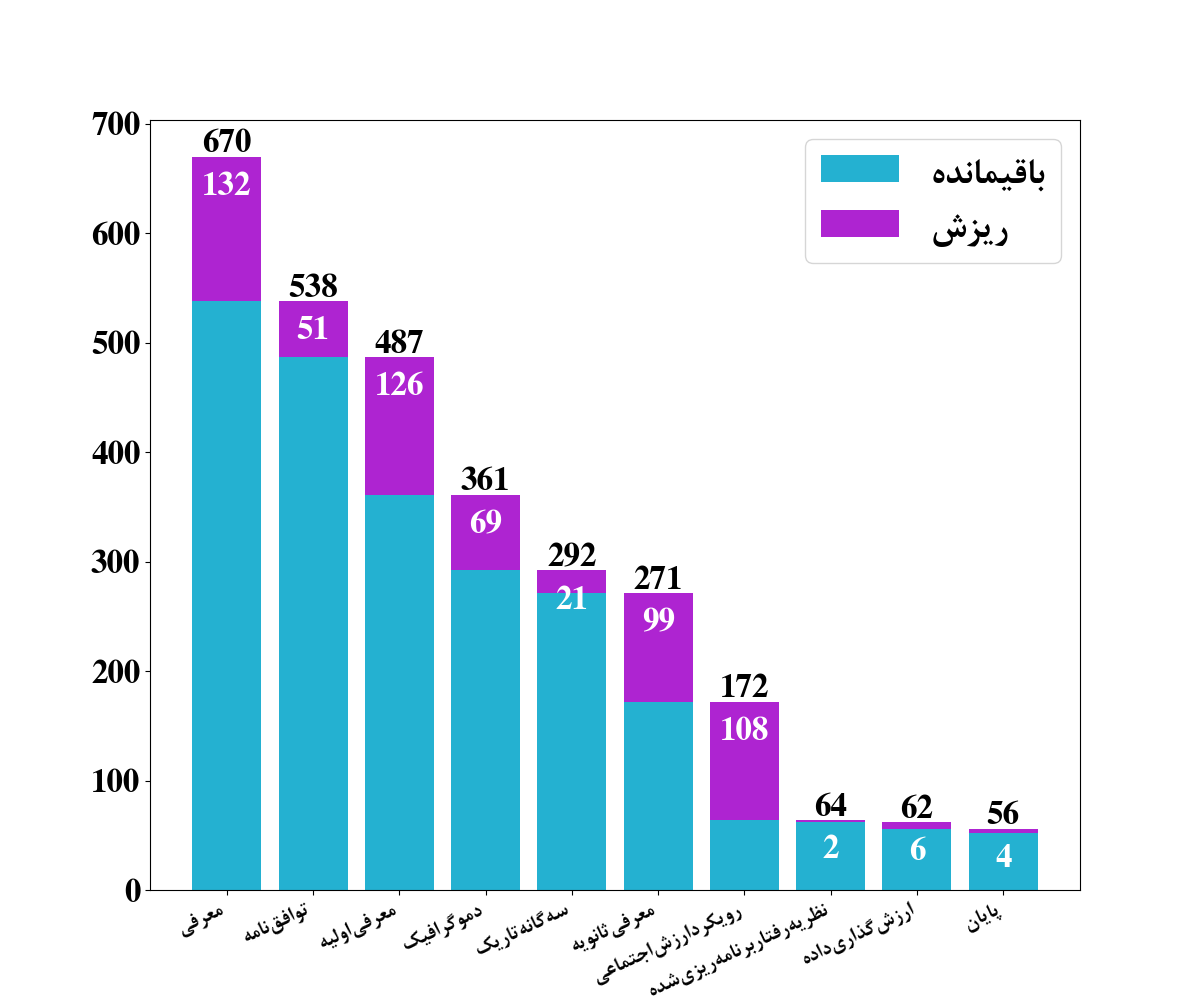
\includegraphics[width=0.8\textwidth]{./img/PageNotSubmitedDataFrame.png}}
    \caption{تعداد ورودی در مقایسه با ریزش‌ها}
    \label{fig:PageNotSubmitedDataFrame}
\end{figure}


% تصویر \label{fig:sexualityAgainstPopulation}

% \begin{figure}[htpb]
%     \centering
%     \includegraphics[width=0.8\textwidth]{./img/sexualityAgainstPopulation.pdf}
%     \caption{فراوانی جنسیت بیان شده در نمونه}
%     \label{fig:sexualityAgainstPopulation}
% \end{figure}

% بعد از حذف داده‌های مربوط به آزمودنی‌هایی که اطلاعات مخدوش یا غیر قابل استفاده داش
% \includepdf[pages={1}]{sexualityAgainstPopulation.pdf}

برای تحلیل رفتار به اشتراک گذاری اطلاعات افرادبالاتر از ۱۸ سال که هر چهار بخش ابتدایی آزمایش شامل
\textit{معرفی اولیه}،
\textit{پرسش‌نامه اول}،
\textit{پرسش‌نامه دوم} و
\textit{معرفی ثانویه}
را کامل کرده بودند، استفاده شد.
از این میان، داده‌های
\BogusEmailDataBogusNoLandingPageDateData
نفر
که فاقد اطلاعات بودند و یا اطلاعات وارد شده توسط آزمودنی
مانند نام و نام‌خانوادگی و شماره تلفن‌ها مخدوش و غیر قابل تشخیص بودند، پاکسازی شدند.

% از این میان داده های افرادی که مشخصات وارد شده توسط آنها مخدوش و غیر صحیح
% بودند، جذف شدند.
 همچنین
$\ValidParticipantsWithBogusPhoneSize$
نفر  از شرکت کنندگان با وجود اینکه
بخش های مختلف آزمایش را به درستی انجام داده بودند، شماره تلفن نامعتبر
برای فرد معرفی شده در بخش‌های
\textit{معرفی اولیه}
و
\textit{معرفی ثانویه}
وارد کرده بودند. همچنین
$1$
نفر دیگر نیز به جای شماره تلفن، ایمیل خود را وارد کرده بود. داده‌های این افراد نیز از نتایج حذف شدند.
داده مربوط به 
$1$
آزمودنی که گزینه عدم تمایل به پاسخ‌گویی برای سوال جنسیت را انتخاب کرده بود، هم به همین ترتیب حذف شد.
در نهایت
$\CleandDataDFForPlotsMinusBogusSize$
باقی ماندند که از این مجموعه داده برای انجام سنجش‌های آماری استفاده شد.
نتایج آماری در بخش دوم آزمایش بر اساس داده‌های موجود و با توجه به ریزش آزمودنی‌های هر مرحله، گزارش شده‌اند.
\section{ویژگی‌های نمونه}
تعداد کل آزمودنی های مجاز برای تحلیل داده در چهار بخش اول آزمایش،
$\CleandDataDFForPlotsMinusBogusSize$
نفر،
با بازه سنی
$\ageMin$
تا
$\ageMax$
و
میانگین
$\sampleAgeMean$
و انحراف استاندارد
$\sampleAgeSD$
بود
\!.
از این میان
$\SampleSizeMale$
نفر مرد و
$\SampleSizeFemale$
زن بودند.
تعداد
$\SampleSizeSexualityNoAnswer$
نفر
نیز از بین گزینه‌های مربوط به جنسیت گزینه عدم تمایل به پاسخگویی را انتخاب کردند
(
تصویر \ref{fig:sexualityAgainstPopulation}
)
\!. 
داده‌های این فرد برای تحلیل‌ استفاده نشده است.

% \begin{figure}[ht]
%     \centerline{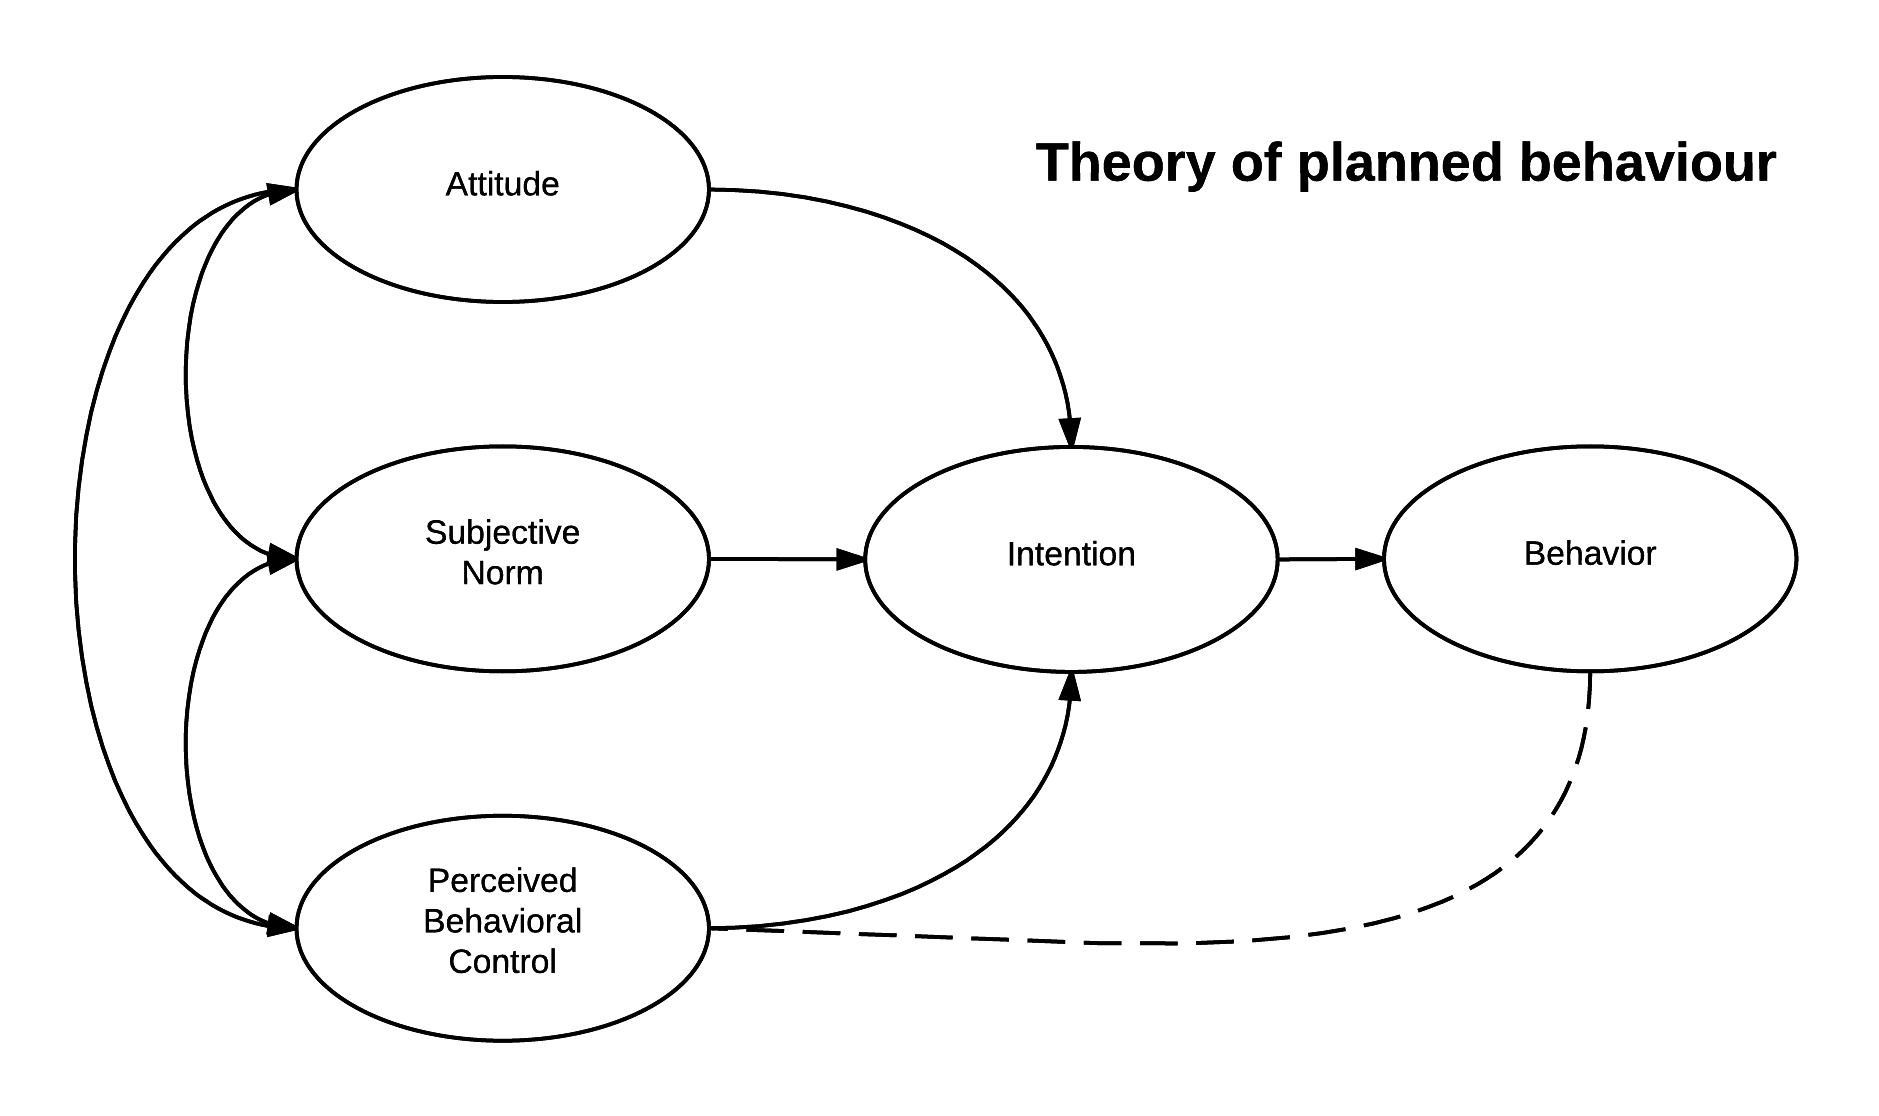
\includegraphics[width=0.8\textwidth]{Theory_of_planned_behavior_chart}}
%     \caption{ساختار نظریه رفتار برنامه ریزی شده
%       %\citep{kim2016integrated}
%     }
%     \label{fig:Theory_of_planned_behavior_chart}
%   \end{figure}\\

% \includepdf[pages={1}]{sexualityAgainstPopulation.pdf}

\begin{figure}[htpb]
    \centering
    \includegraphics[width=0.8\textwidth]{./img/sexualityAgainstPopulation.pdf}
    \caption{فراوانی جنسیت بیان شده در نمونه}
    \label{fig:sexualityAgainstPopulation}
\end{figure}
\begin{figure}[htpb]
    \centering
    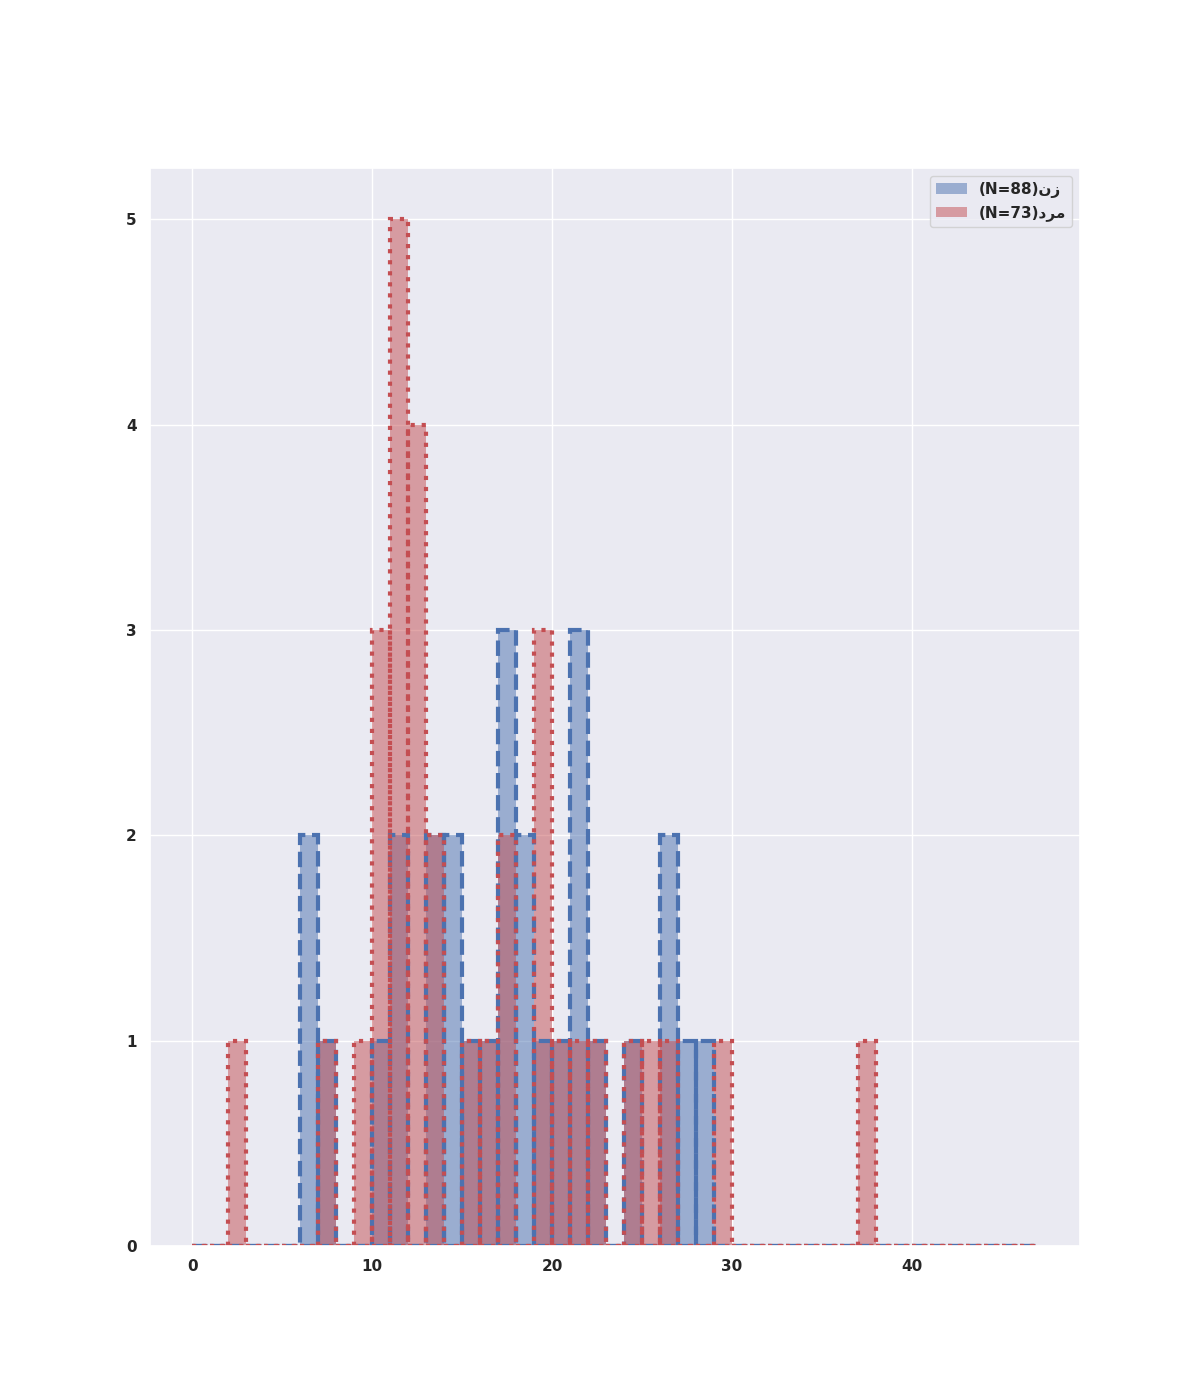
\includegraphics[width=0.8\textwidth]{./img/BoxPlotDTRSVOType.png}
    \caption{نمودار مقایسه‌ای هیستوگرام سه‌گانه تاریک بر اساس جنسیت}
    \label{fig:BoxPlotDTRSVOType}
\end{figure}
\begin{figure}[htpb]
    \centering
    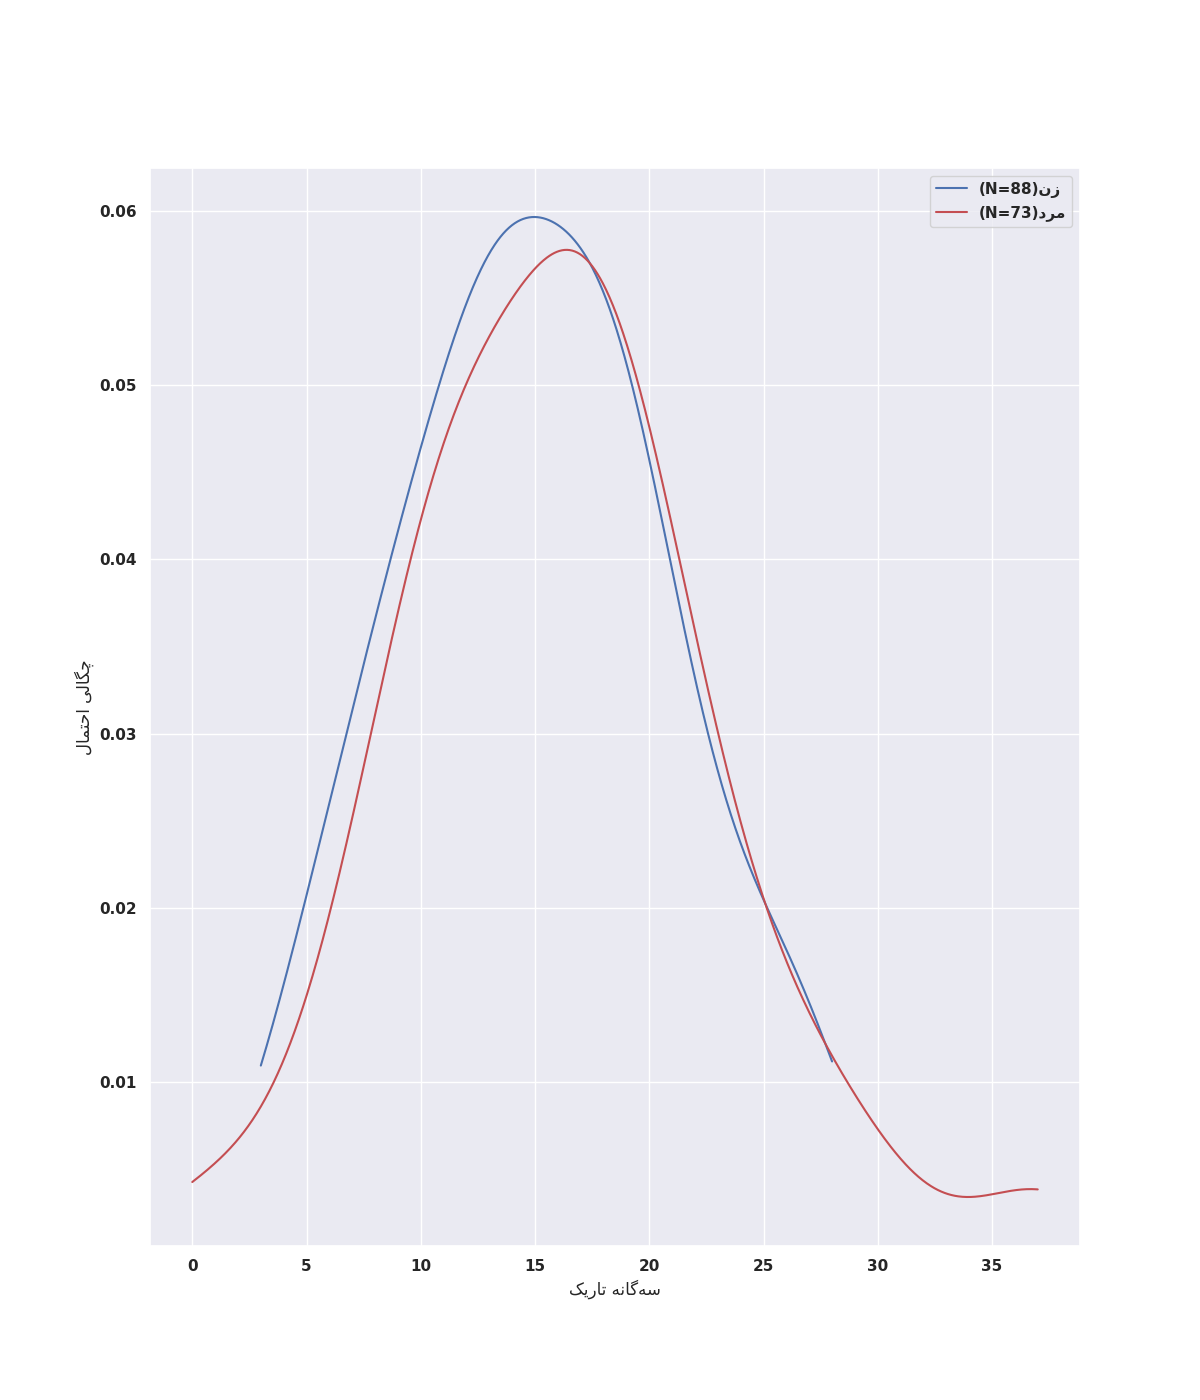
\includegraphics[width=0.8\textwidth]{./img/PDFGramDTRSex.png}
    \caption{نمودار مقایسه‌ای توزیع چگالی احتمال سه‌گانه تاریک بر اساس جنسیت}
    \label{fig:PDFGramDTRSex}
\end{figure}


% \section{سه‌گانه تاریک}
% جدول
% \CompareDarkTriadStatisticsRef
% به صور مقایسه‌ای
% شاخص‌های آماری میانگین و انحراف‌معیار به دست آمده در پرسش‌نامه پیاده شده در این آزمایش
% را با آزمایش‌های پیشین نمایش می‌دهد.

% \CompareDarkTriadStatisticsCustomTableCommand


% \begin{landscape}
% \StyledTableFromDFCommand
% \end{landscape}
\section{پرسشنامه اطلاعات دموگرافیک}

\eqref{tab:LatexFromStatisticsRankMeans}

\LatexFromStatisticsRankMeansCommand
% \includepdf[pages={1}]{./img/CorrPlotIntervals.pdf}
\begin{figure}[htpb]
    \centering
    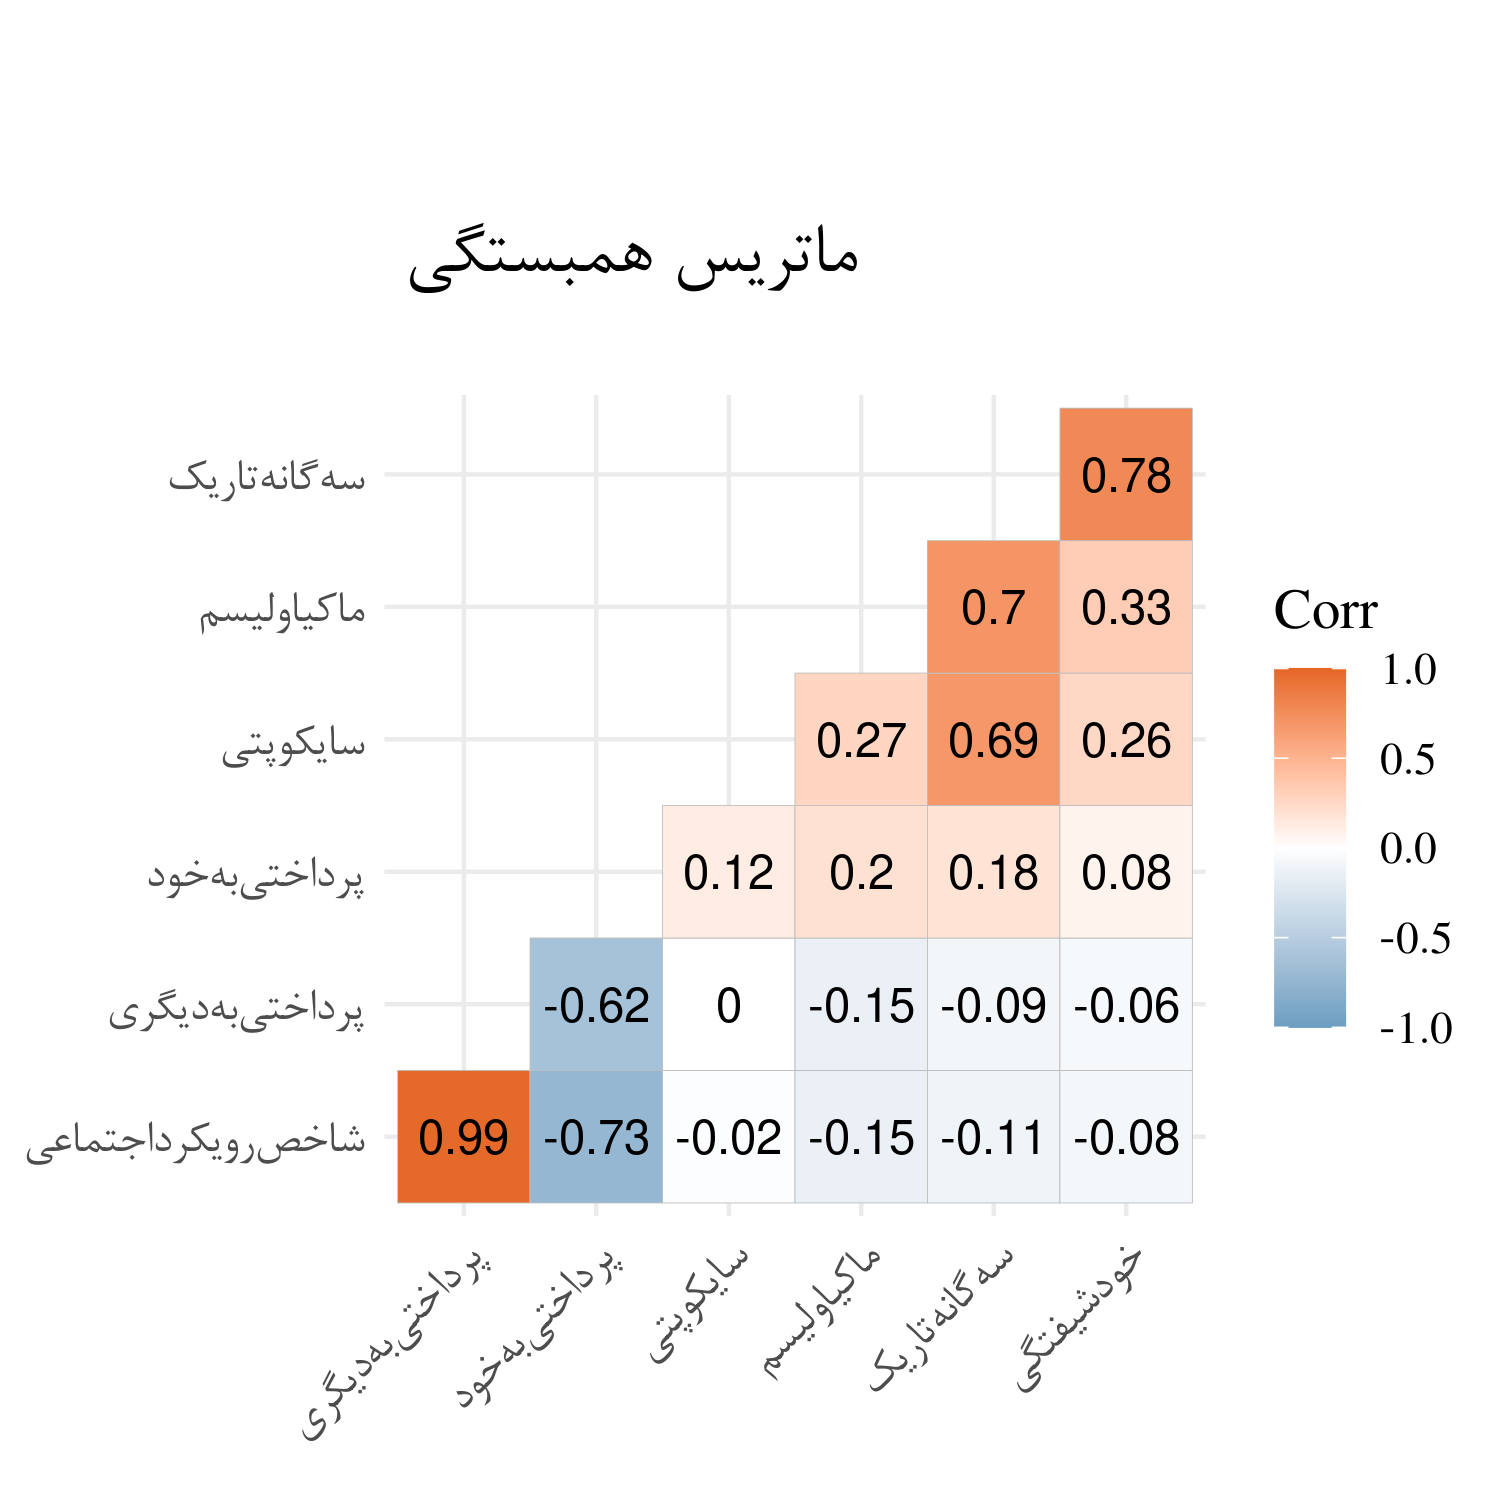
\includegraphics[width=0.8\textwidth]{./img/CorrPlotIntervals.png}
    \caption{ماتریس همبستگی}
    \label{fig:CorrPlotIntervals}
\end{figure}

% \subsection{نتایج آزمون جهت‌گیری ارزش اجتماعی}
\section{نتایج آزمون جهت‌گیری ارزش اجتماعی}
از میان همه شرکت کنندگان
\noOfIndividualisticParticipants
نفر در دسته
\textit{
    \gls{Individualistic}
}
،
% \noOfCompetitiveParticipants
% نفر در دسته
% \textit{
%     \gls{Competitive}
% }
% ،
\noOfCooperativeParticipants
نفر در دسته
\textit{
    \gls{Prosocial}
}\!(\textit{
    \gls{Cooperative}
})
و
\noOfAltruisticParticipants
نفر در دسته
\textit{
    \gls{Altruistic}
}
قرار داشتند.
تعداد افراد دسته‌های دیگر
\!(\!\textit{
    \gls{Martyrdom}
}،
\textit{
    \gls{Masochism}
}،
\textit{
    \gls{Sadomasochism}
} و
\textit{
    \gls{Competitive}
}\!)
در نمونه جمع‌آوری‌شده صفر بود.
نمودار \ref{fig:SVOAgainstPopulationBarPlot}
فراوانی دسته‌های رویکرد ارزش اجتماعی در نمونه را نشان می‌دهد. این نمودار بر اساس حجم نمونه‌ای که 
بخش رویکرد ارزش اجتماعی را انجام داده اند ترسیم شده است
($N=\SVOSliderTestDropsPageRemainers$).

\begin{figure}[htpb]
    \centering
    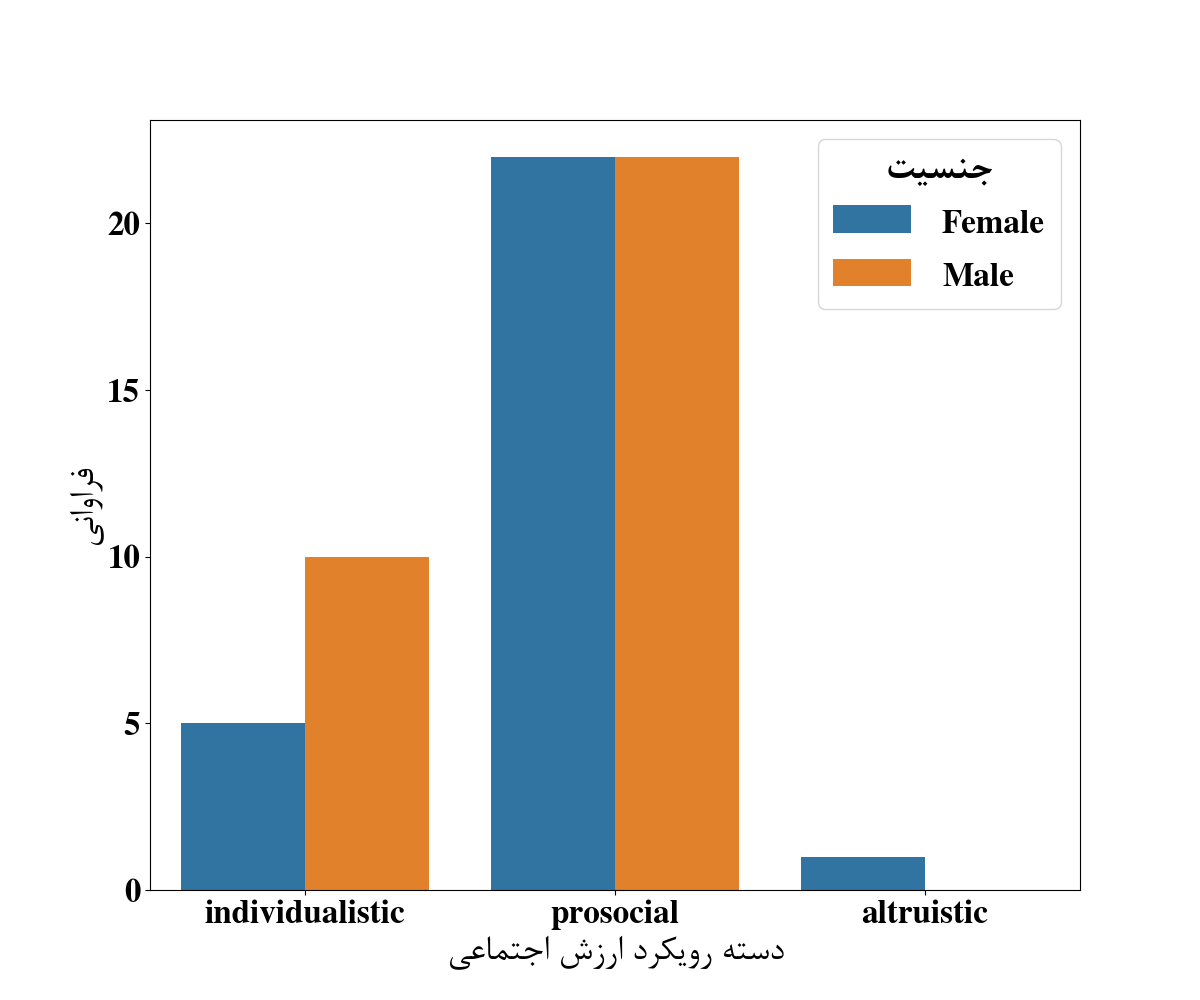
\includegraphics[width=0.8\textwidth]{./img/SVOAgainstPopulationSexBarPlot.png}
    \caption{فراوانی دسته‌های رویکرد ارزش اجتماعی بر اساس جنسیت}
    \label{fig:SVOAgainstPopulationSexBarPlot}
\end{figure}
\begin{figure}[htpb]
    \centering
    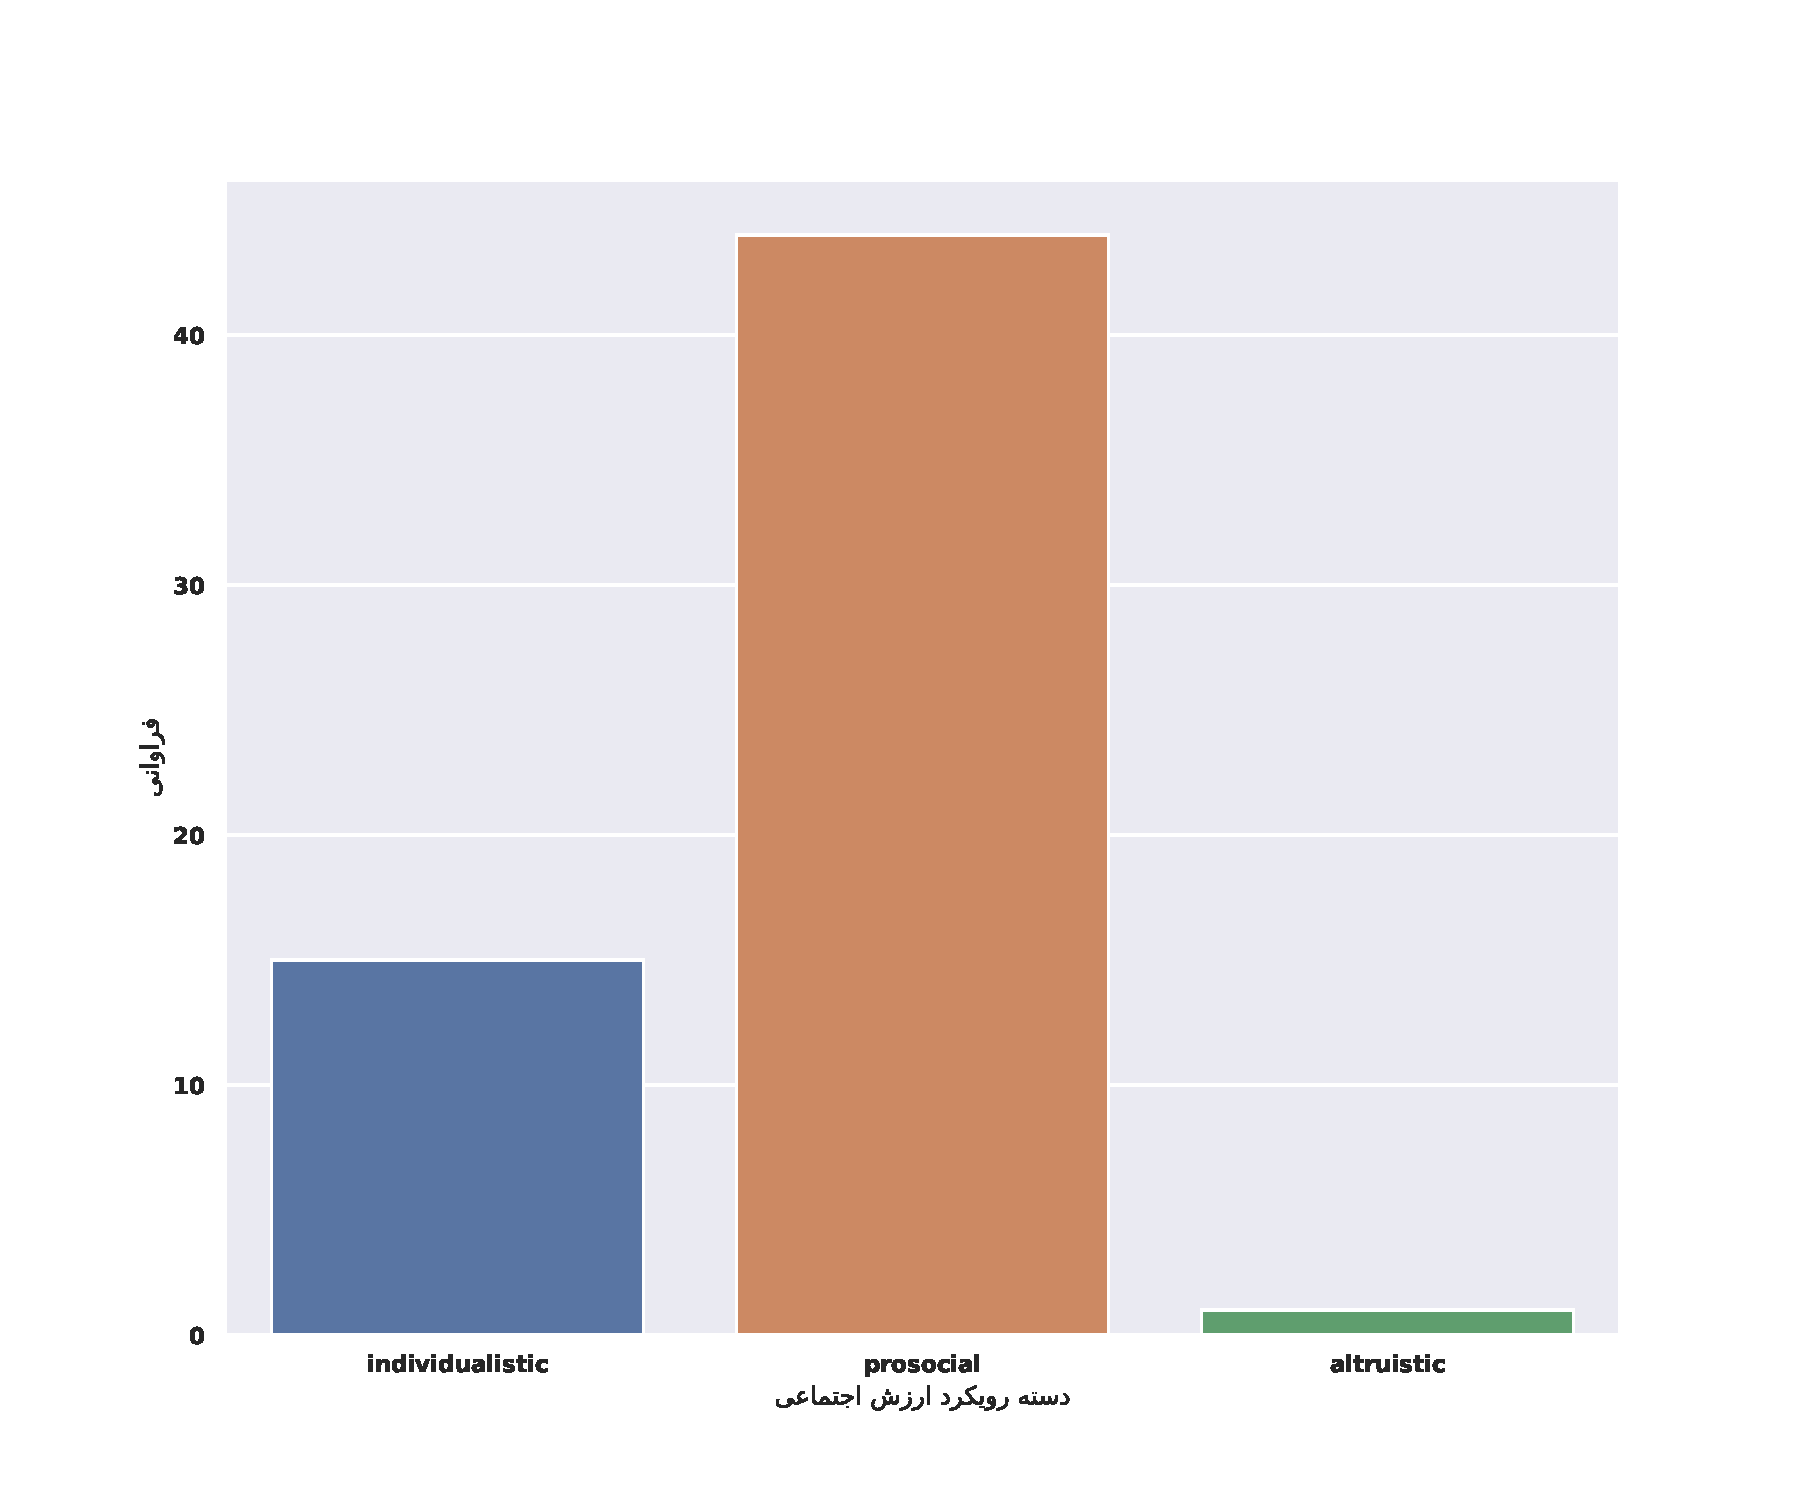
\includegraphics[width=0.8\textwidth]{./img/SVOAgainstPopulationBarPlot.pdf}
    \caption{فراوانی دسته‌های رویکرد ارزش اجتماعی}
    \label{fig:SVOAgainstPopulationBarPlot}
\end{figure}
\section{تغییر در رفتار
\!(قبل و بعد از پرسشنامه دموگرافیک و سه‌گانه‌تاریک و تحت تاثیر تطمیع 
)}

\begin{table}
    \begin{center}
        \caption{More columns.}
        \label{tab:table1}
        \begin{tabular}{|r|L|L|}
دسته & میانگین & انحراف‌معیار & \\ % <-- added & and content for each column
            \hline
            1                & \XYNullDarkTriadXX           &  \textit{\gls{XX}}             \\ % <--
            2                & \XYNullDarkTriadXY             &  \textit{\gls{NullX}}               \\ % <--
            3                & \XYNullDarkTriadNullX        &  \textit{\gls{NullNull}}             \\ % <--
            3                & \XYNullDarkTriadXNull        &  \textit{\gls{NullNull}}             \\ % <--
            3                & \XYNullDarkTriadNullNull        &  \textit{\gls{NullX}}                 % <--
        \end{tabular}
    \end{center}
\end{table}

در
تصویر \ref{fig:FrequencyBehaviorPhoneNumber}
اطلاعات تغییر رفتار
مشخص است.

برای ایجاد تغییر رفتار در آزمودنی از 
\!\textit{
    \gls{Temptation}
}
استفاده شد
\citep{maihaniemiCompetitionLawBig2020}.
\begin{figure}[htpb]
    \centering
    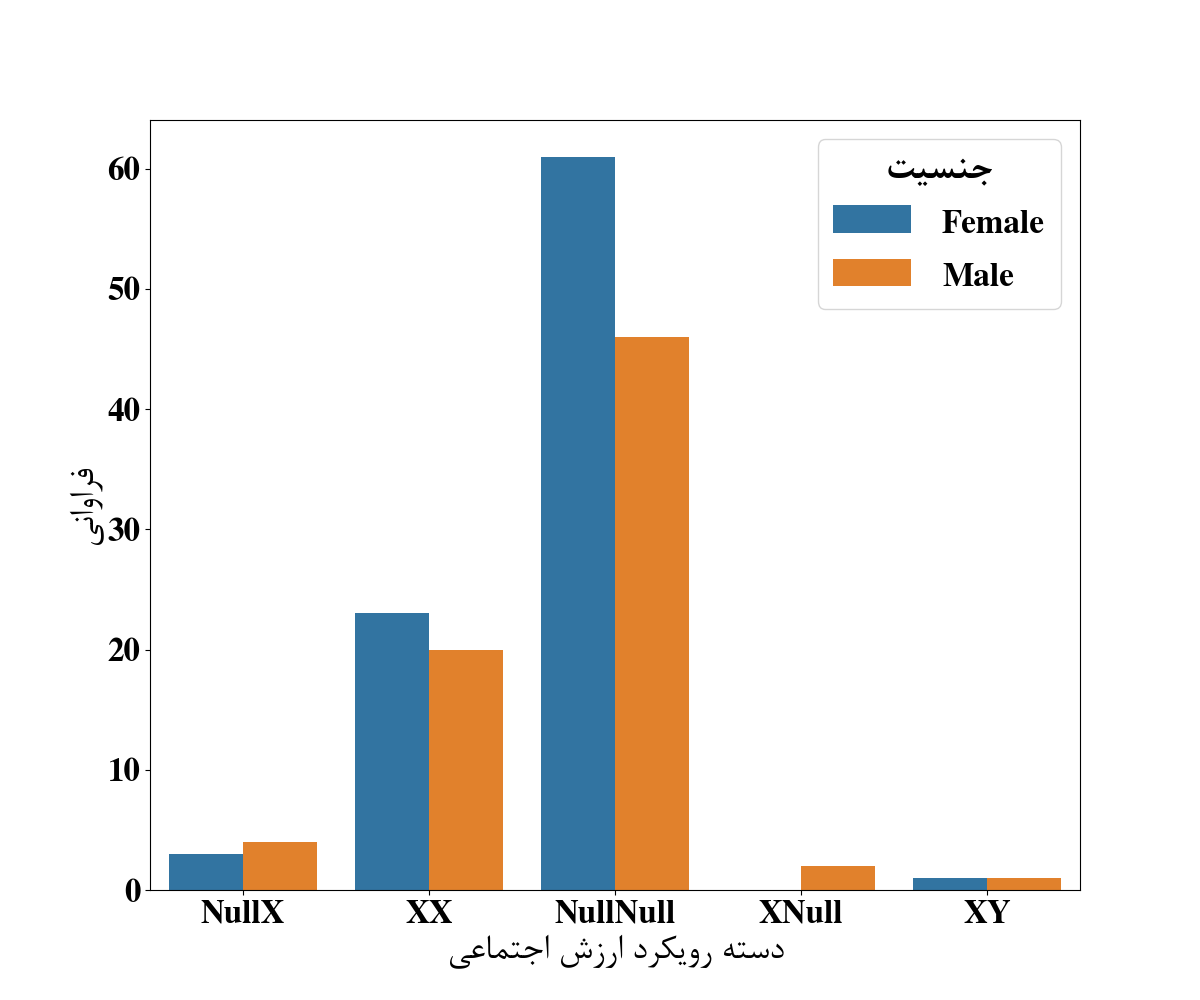
\includegraphics[width=0.8\textwidth]{./img/FrequencyBehaviorPhoneNumber.png}
    \caption{فراوانی دسته‌بندی‌های تغییر رفتار بر اساس جنسیت}
    \label{fig:FrequencyBehaviorPhoneNumber}



نمودار 
\ref{fig:BehavioralChange_DarkTriad_Boxplot}
تفاوت نمره سه‌گانه تاریک را در دسته‌های پنجگانه تغییر رفتار  را نشان می‌دهد.

\end{figure}
\begin{figure}[htpb]
    \centering
    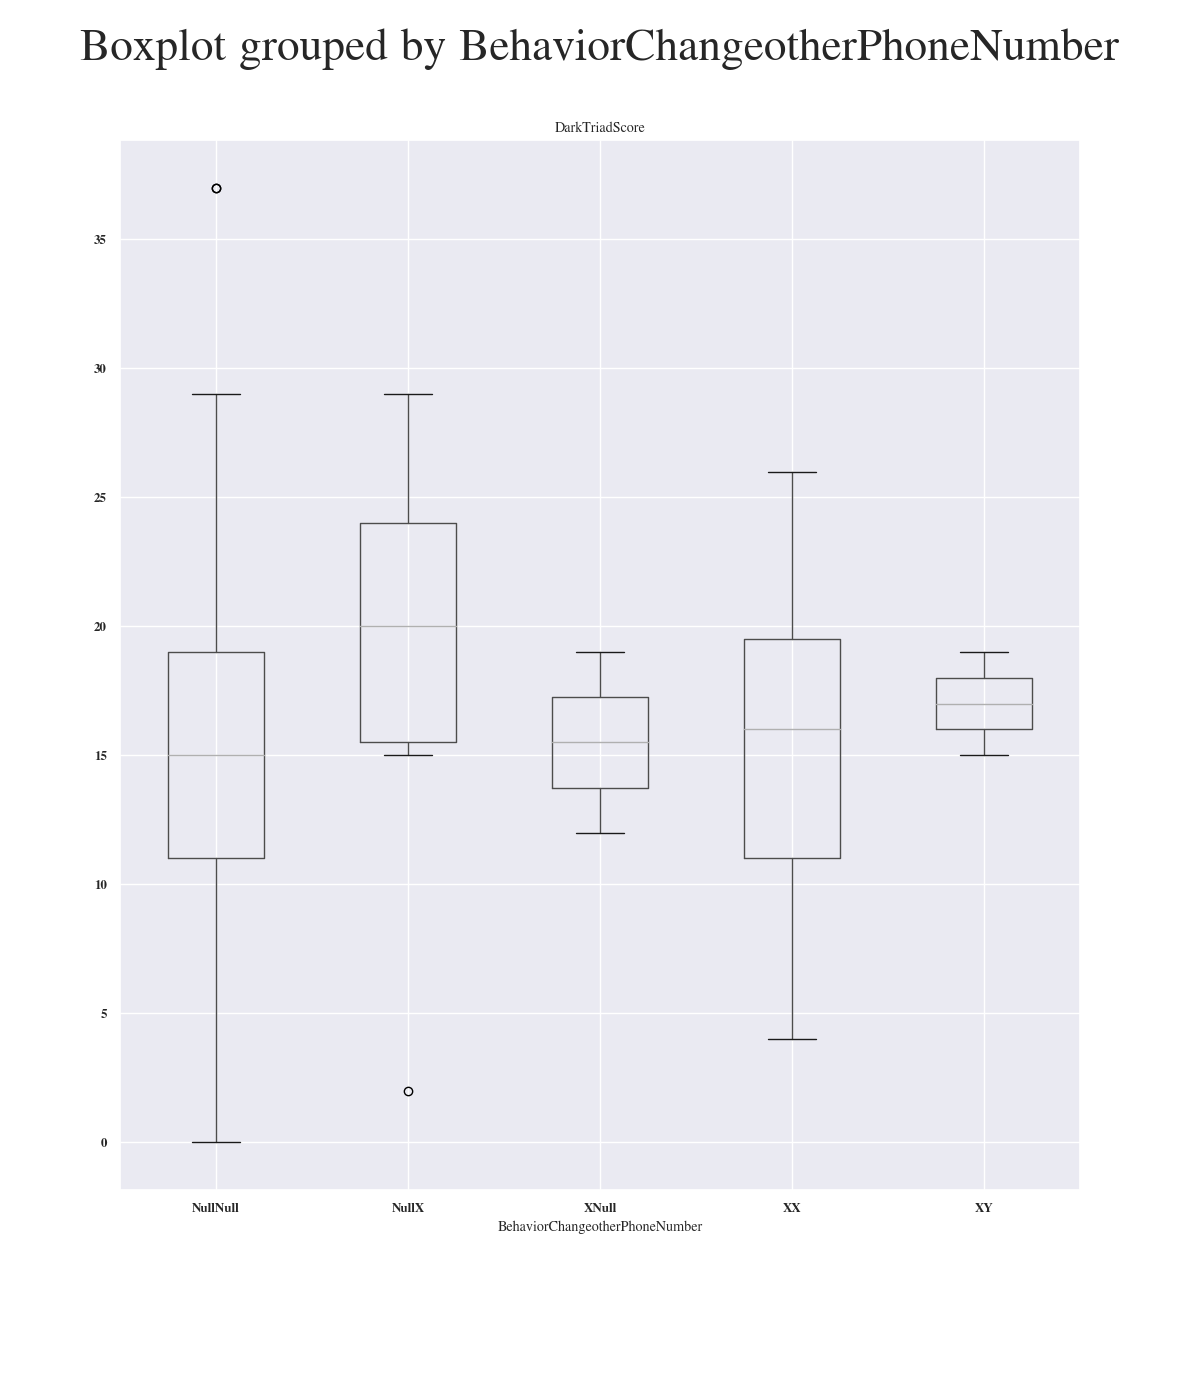
\includegraphics[width=0.8\textwidth]{./img/BehavioralChange_DarkTriad_Boxplot.png}
    \caption{نمودار جعبه‌ای دسته‌های تغییر رفتار بر اساس سه‌گانه تاریک}
    \label{fig:BehavioralChange_DarkTriad_Boxplot}
\end{figure}

برای بررسی تفاوت میان گروه‌هایی که تعداد آزمودنی آنها برای انجام آزمون آماری کافی بود از تی-تست استفاده شد. 
میان نمره سه‌گانه تاریک افرادی که دارای تغییر رفتار
\textit{\gls{XX}}
و 
\textit{\gls{NullX}}
بودند تفاوتی مشاهده نشد
(\XYNullDarkTriadXXXYNullDarkTriadNullXTTestPValueReport)
میان نمره سه‌گانه تاریک افرادی که دارای تغییر رفتار
\textit{\gls{XX}}
و 
\textit{\gls{NullNull}}
بودند تفاوتی مشاهده نشد
(\XYNullDarkTriadXXXYNullDarkTriadNullNullTTestPValueReport)
میان نمره سه‌گانه تاریک افرادی که دارای تغییر رفتار
\textit{\gls{NullNull}}
و 
\textit{\gls{NullX}}
بودند تفاوتی مشاهده نشد
(\XYNullDarkTriadNullXXYNullDarkTriadNullNullTTestPValueReport)





% \begin{figure}[htpb]
%     \centering
%     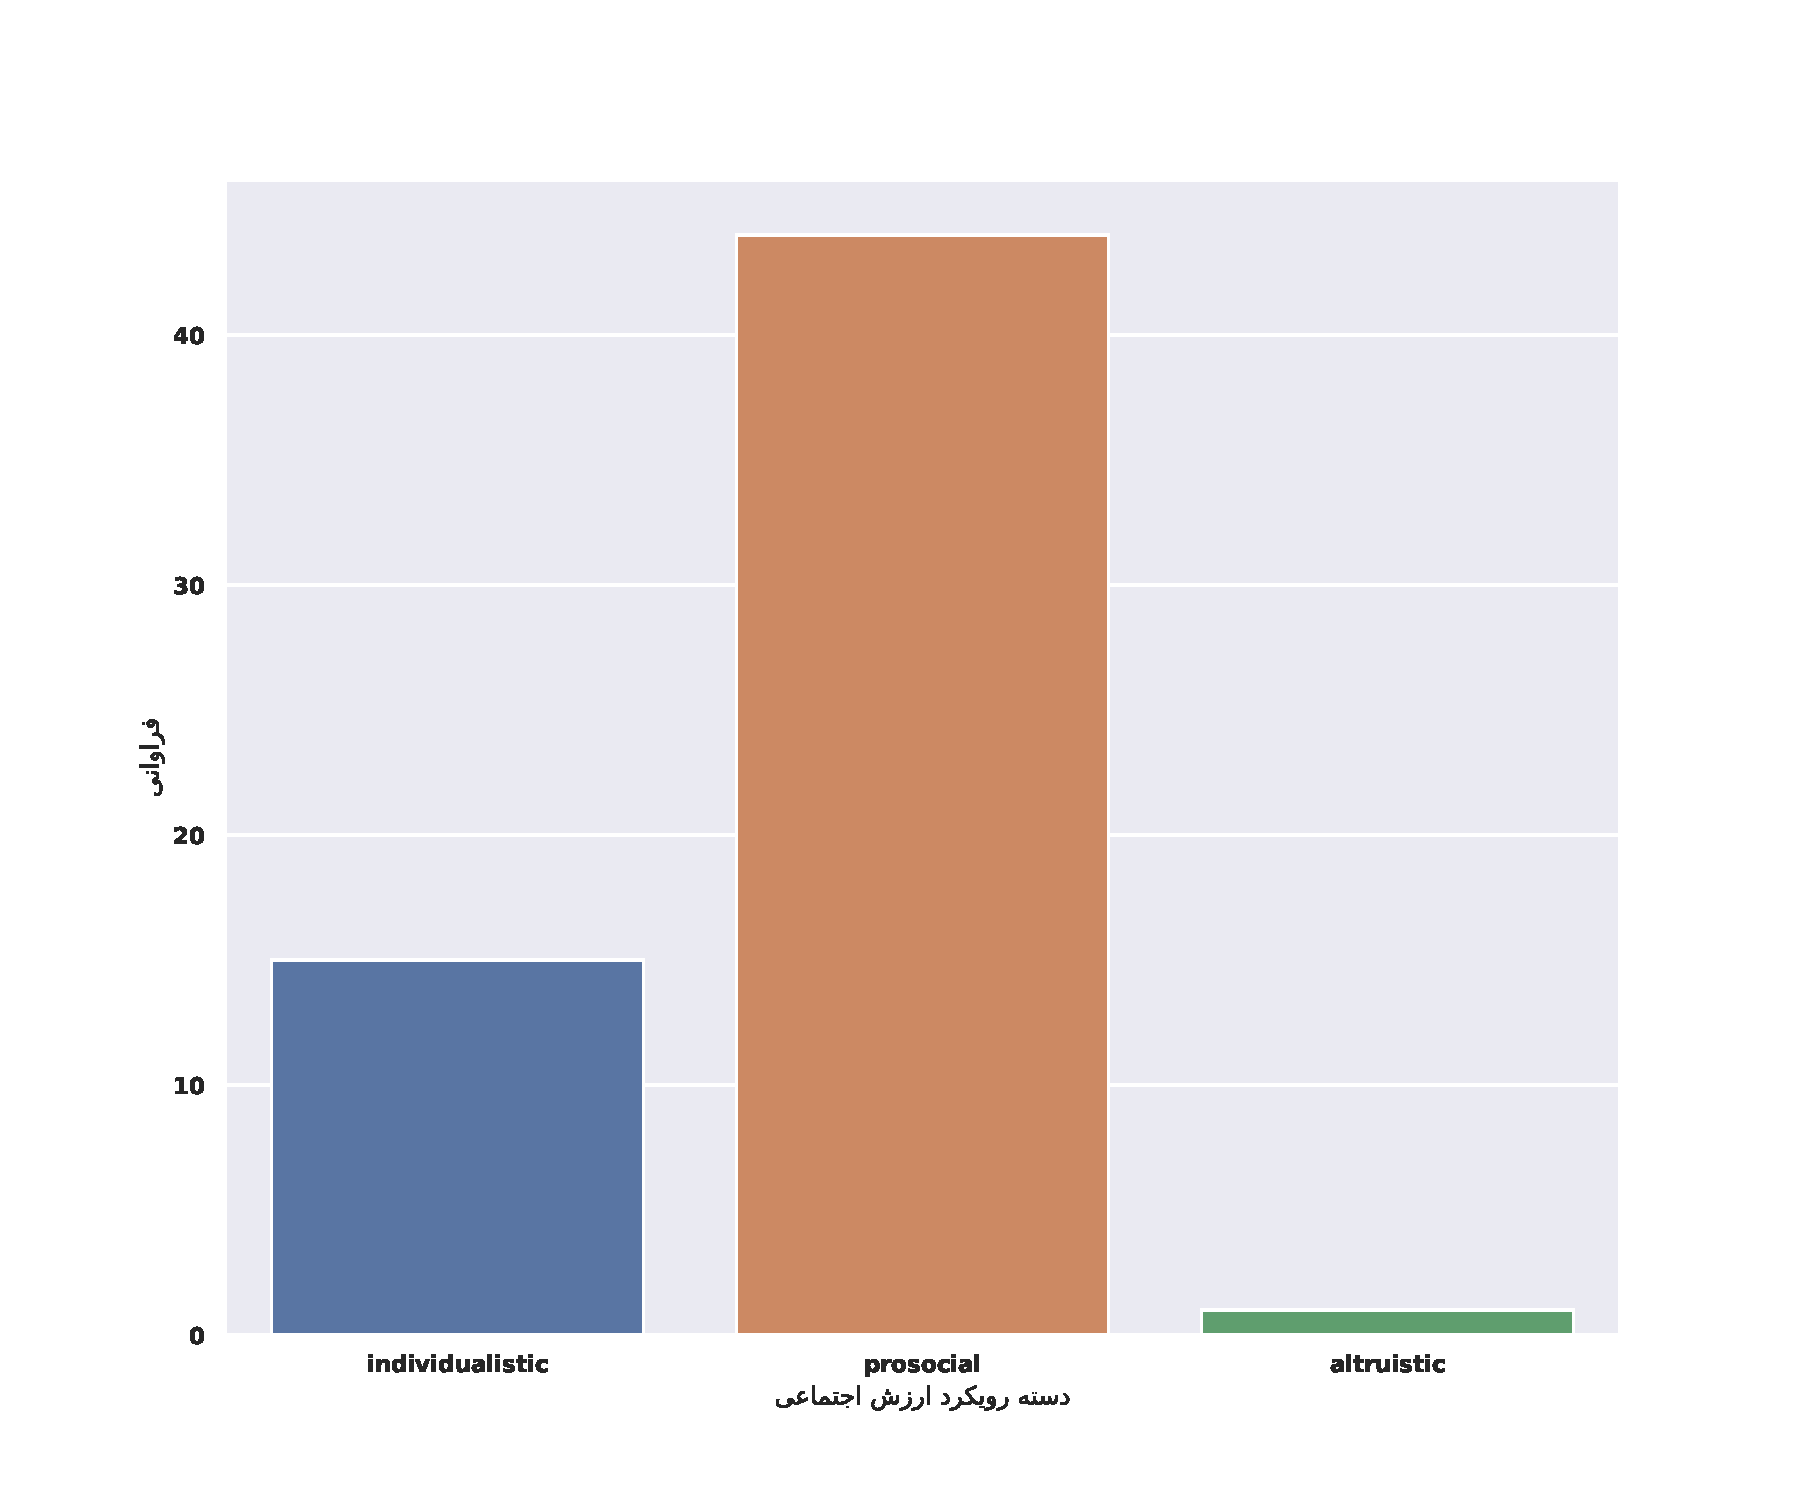
\includegraphics[width=0.8\textwidth]{./img/SVOAgainstPopulationBarPlot.pdf}
%     \caption{فراوانی دسته‌های رویکرد ارزش اجتماعی}
%     \label{fig:SVOAgainstPopulationBarPlot}
% \end{figure}


% \begin{figure}[htpb]
%     \centering
%     
\includegraphics[width=0.8\textwidth]{./img/SVOAgainstPopulation.pdf}
%     \caption{فراوانی دسته‌های رویکرد ارزش اجتماعی}
%     \label{fig:SVOAgainstPopulation}
% \end{figure}
% میانگین کلی نمره‌ای که همه آزمودنی‌ها در هر دو گروه به ۱۴ سوال هر دو دسته
% نمرات از دید خود
% \!(باور به ارزش اطلاعات)
% $\meanOfSelfWTPAllTwoParticipantGroupsAllTwoQuestionSection$
% با انحراف استاندارد
% $\SDOfSelfWTPAllTwoParticipantGroupsAllTwoQuestionSection$
% و از دید دیگران
% $\meanOfOtherWTPAllTwoParticipantGroupsAllTwoQuestionSection$
% \!(باور هنجاری به ارزش اطلاعات)
% با انحراف استاندارد
% $\SDOfOtherWTPAllTwoParticipantGroupsAllTwoQuestionSection$
% بود.

\section{نتایج آزمون‌های آماری سه‌گانه‌تاریک و رویکرد‌ارزش‌اجتماعی}

نمره سه‌گانه تاریک در دو گروه  فرد‌گرا و جامعه‌پسند دارای تفاوت معنادار نبود
% (\!\BoxPlotDTRSVOTypeProsocialBoxPlotDTRSVOTypeIndivisualistTTESTIndPValueReport)
(شکل 
\ref{fig:BoxPlotDTRSVOTypeProsocialBoxPlotDTRSVOTypeIndivisualistTTESTIndPValueReport}).

\begin{figure}[htpb]
    \centering
    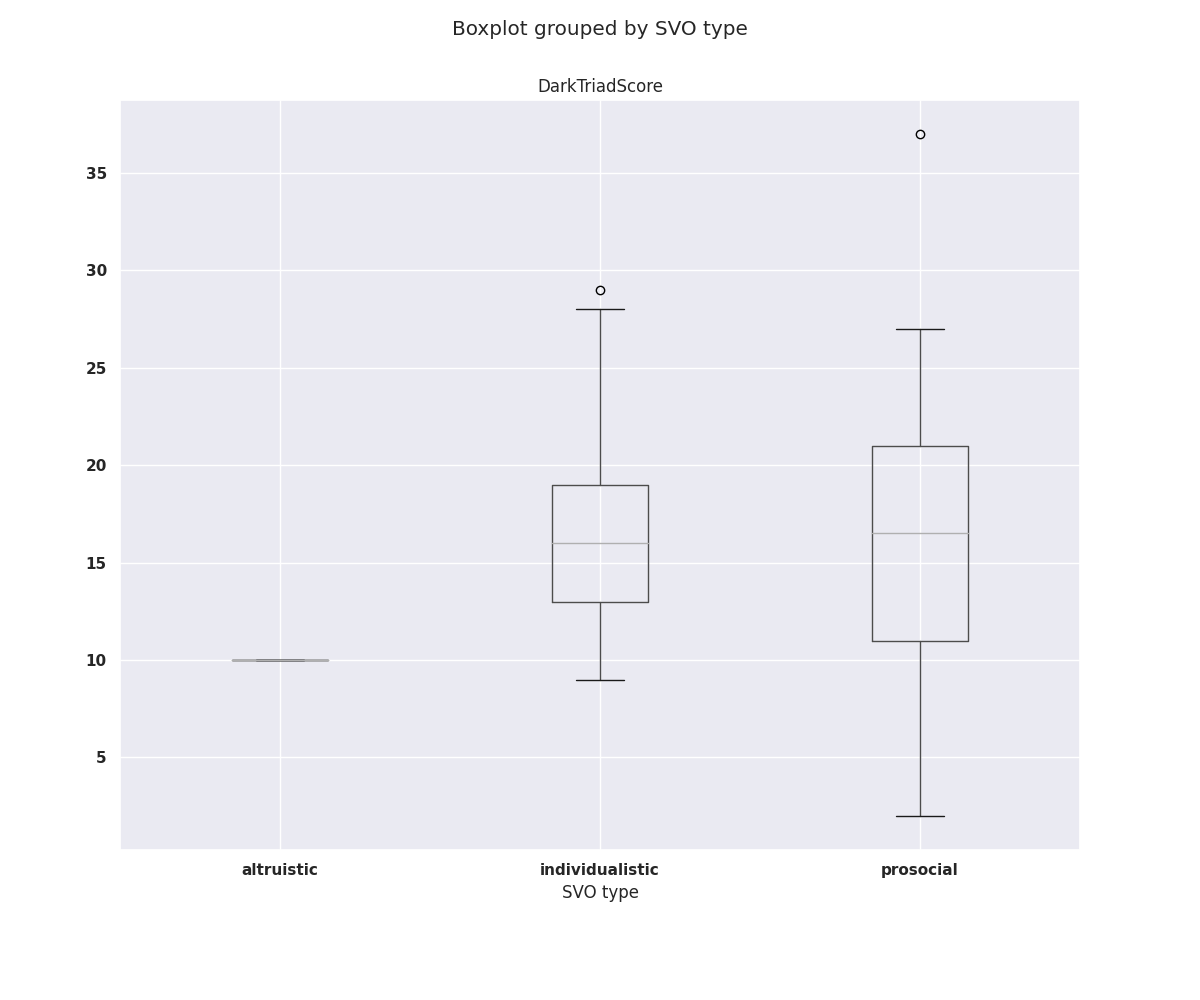
\includegraphics[width=0.8\textwidth]{./img/BoxPlotDTRSVOTypeProsocialBoxPlotDTRSVOTypeIndivisualistTTESTIndPValueReport.png}
    \caption{نمودار جعبه‌ای نمره سه‌گانه تاریک در گروه‌های جامعه‌پسند و فرد‌گرا}
    \label{fig:BoxPlotDTRSVOTypeProsocialBoxPlotDTRSVOTypeIndivisualistTTESTIndPValueReport}
\end{figure}

\begin{figure}[htpb]
    \centering
    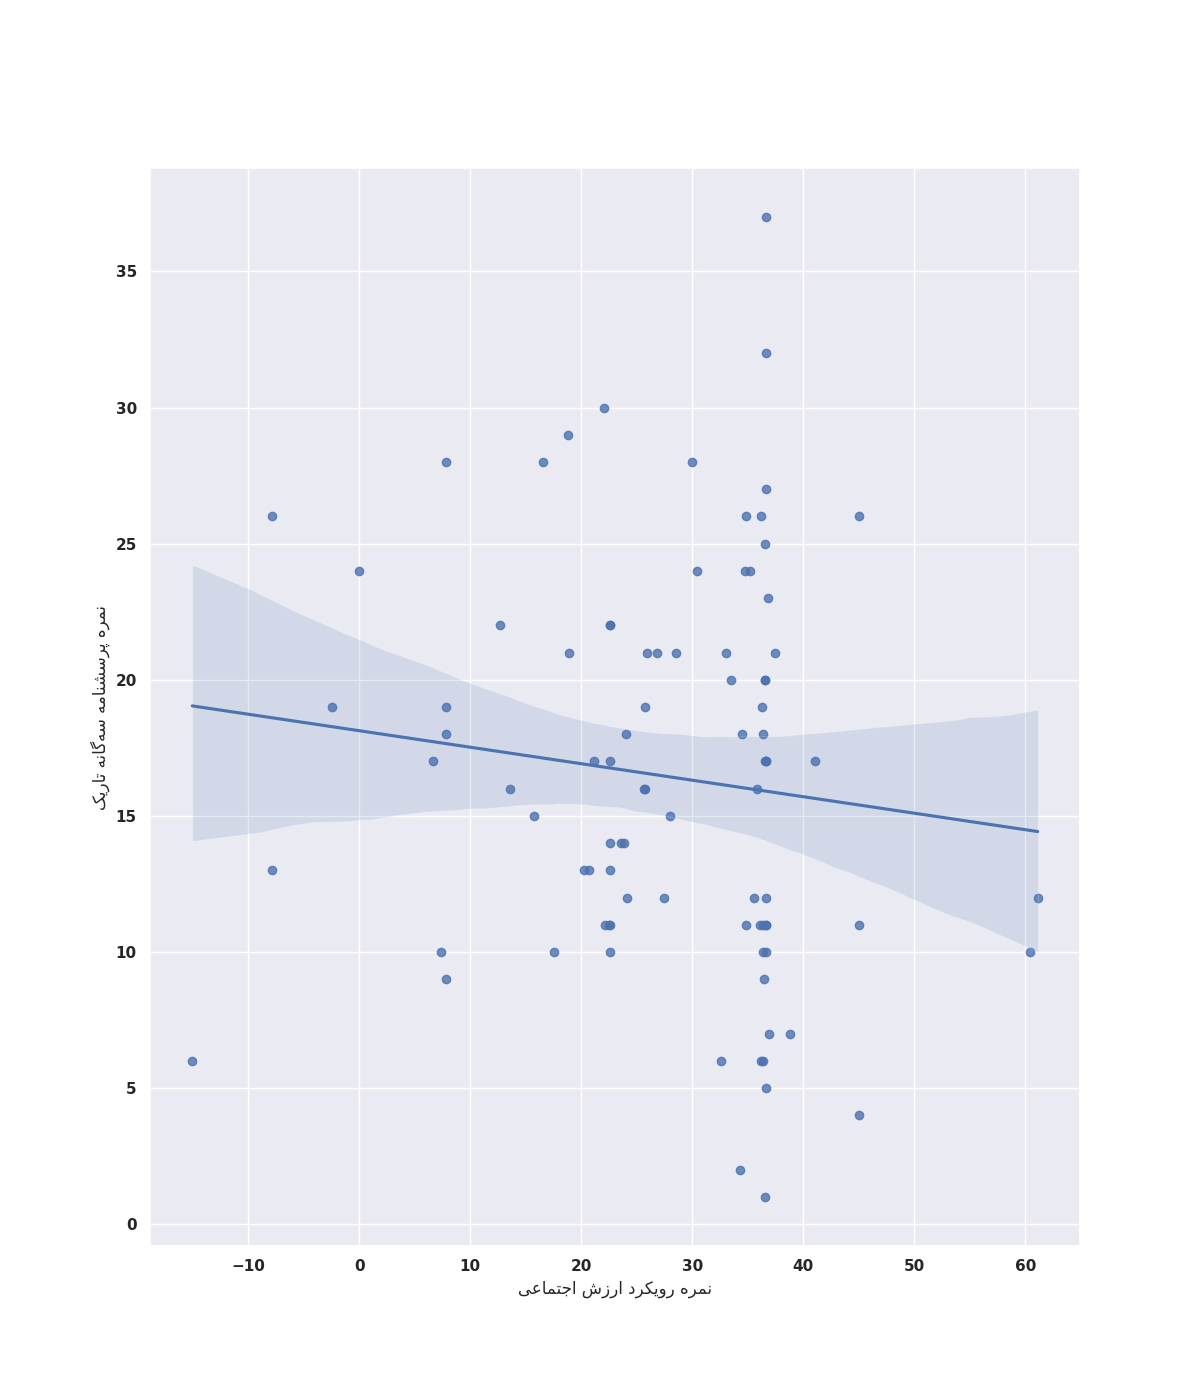
\includegraphics[width=0.8\textwidth]{./img/ScatterSVOScoreDarkTriadScoreSNS.png}
    \caption{نمودار پراکنش نمره رویکرد ارزش اجتماعی  نسبت به نمره سه‌گانه تاریک}
    \label{fig:ScatterSVOScoreDarkTriadScoreSNS}
\end{figure}
\begin{figure}[htpb]
    \centering
    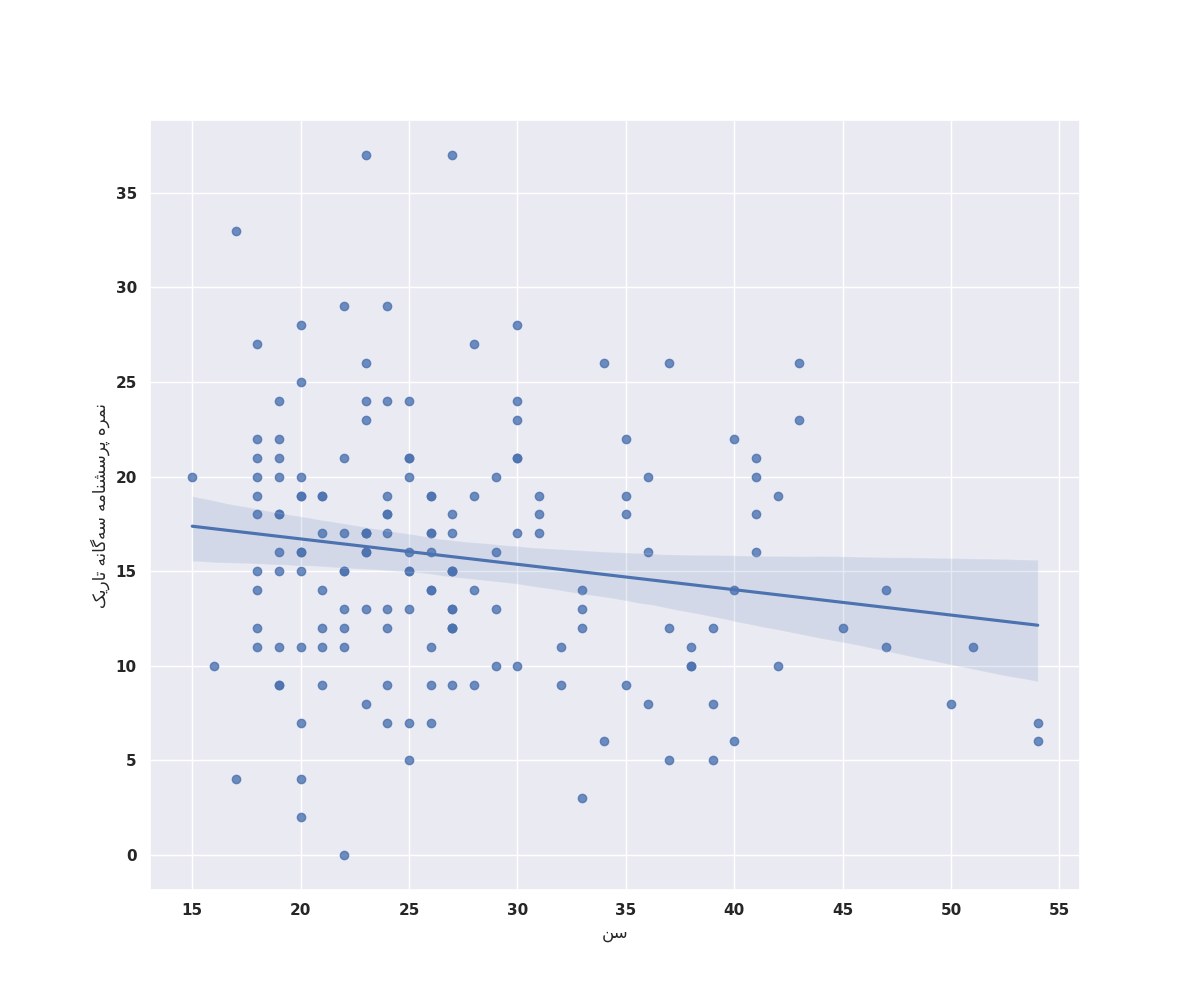
\includegraphics[width=0.8\textwidth]{./img/ScatterDTRAgeSNS.png}
    \caption{نمودار پراکنش و مدل رگرسیونی سن نسبت به نمره سه‌گانه تاریک}
    \label{fig:ScatterDTRAgeSNS}
\end{figure}
در شکل
\ref{fig:ScatterDTRAgeSNS}
نمودار پراکنش و مدل رگرسیونی سن نسبت به نمره سه‌گانه تاریک مشخص شده‌است.
شکل
\ref{fig:ScatterSVOScoreDarkTriadScoreSNS}
نمودار پراکنش نمره رویکرد ارزش اجتماعی را نسبت به نمره سه‌گانه تاریک نشان می دهد.
و در شکل
\ref{fig:DTRHistogram}
فراوانی نمره‌های پرسش‌نامه سه‌گانه تاریک مشخص شده است.

\begin{figure}[htpb]
    \centering
    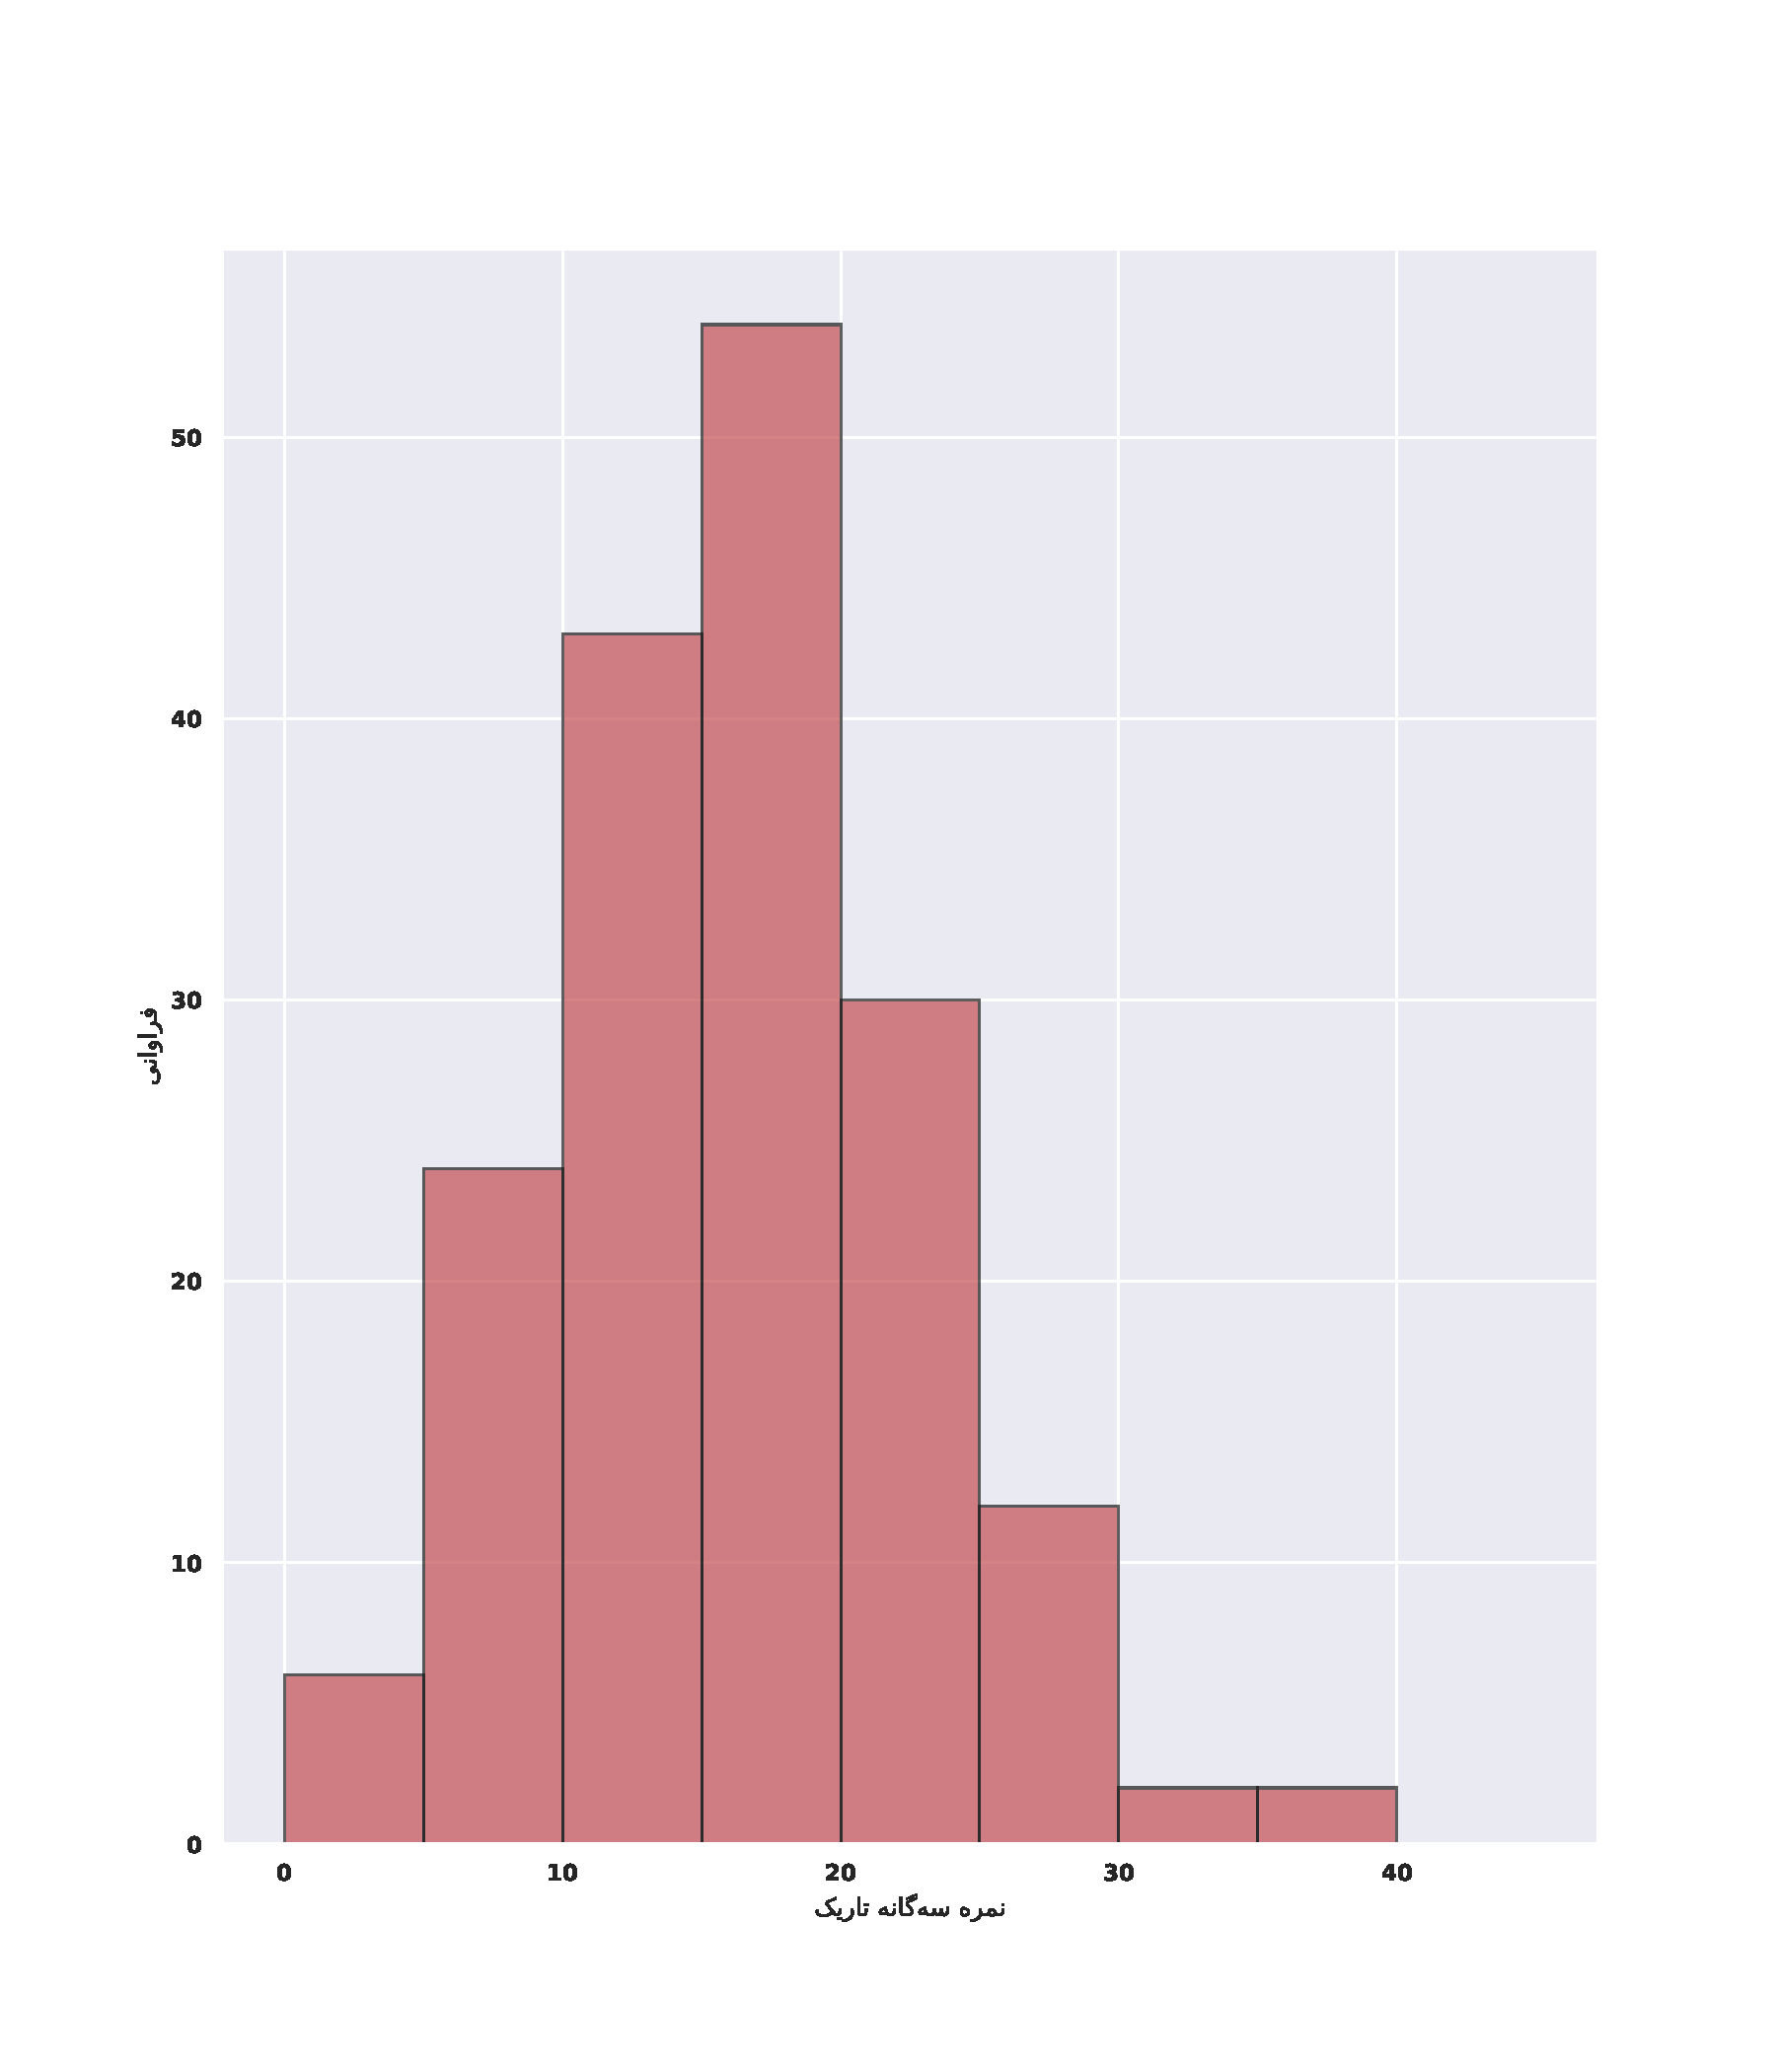
\includegraphics[width=0.8\textwidth]{./img/DTRHistogram.pdf}
    \caption{نمودار هیستوگرام نمره  سه‌گانه تاریک}
    \label{fig:DTRHistogram}
\end{figure}

\section{نمره سه‌گانه تاریک در زنان و مردان}
 تفاوت معنی داری بین نمرات زنان 
 ($Mean=\DTRFemaleMean,N=\DarkTriadScoreSexGroupByFemaleSize$)
 و مردان 
 ($Mean=\DTRMaleMean,N=\DarkTriadScoreSexGroupByMaleSize$)
 در آزمون سه‌گانه تاریک مشاهده نشده
\!(\DarkTriadScoreSexIndTTestPValue)
\!(نمودار
\ref{fig:BoxPlotDarkTriadScoreSex}
).

\begin{figure}[htpb]
    \centering
    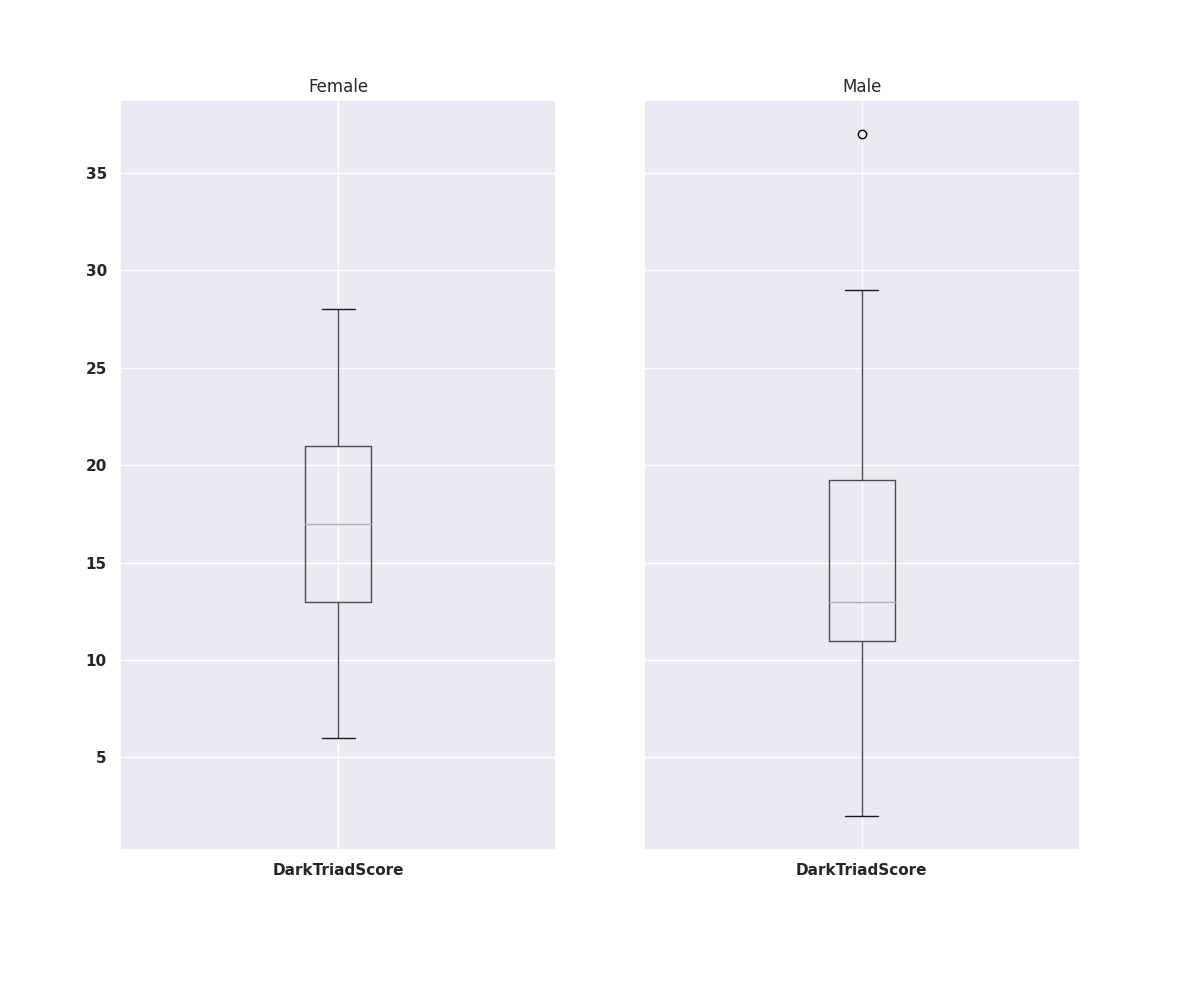
\includegraphics[width=0.8\textwidth]{./img/BoxPlotDarkTriadScoreSex.png}
    \caption{نمودار جعبه‌ای نمره سه‌گانه تاریک بر اساس جنسیت}
    \label{fig:BoxPlotDarkTriadScoreSex}
\end{figure}

% \section{سیاهه ارزش‌گذاری مجموعه‌داده}
% در این پژوهش از
% % سیاهه ارزش‌گذاری مجموعه‌داده
% {\textit{\gls{Dataset valuation invetory}}}
% که یک
% {\textit{\gls{The researcher made a questionnaire}}}
% است برای اندازه‌گیری
% \gls{Attitude}
% نسبت به ارزش دسته‌های مختلف اطلاعات شخصی، استفاده شده است.
% هر   آزمودنی‌ در هر
% \textit{\gls{Trial}}
% به
% \textit{\gls{Dataset}}
% ارائه شده عددی از بازه صفر تا ۱۰۰ نسبت داده است. این عدد به عنوان مقیاسی از
% %  ارزش ذهنی
% \textit{\gls{Subjective value}}
% دسته‌ای از اطلاعات که
% \textit{\gls{Trial}}
% به آن تعلق دارد، تلقی می‌شود.

% همزمان با شروع
% \textit{\gls{Online survey}}
% در بخش دریافت
% \textit{\gls{Consent}}
% آزمودنی‌ها به طور تصادفی و از طریق کد
% \textit{\gls{JavaScript}}
% اجرا شده در
% \textit{\gls{Browser}}
% به دو دسته تقسیم شدند.

% \begin{table}[h!]
%     \begin{center}
%         \caption{More columns.}
%         \label{tab:table1}
%         \begin{tabular}{l|c|r|l}
%             \textbf{Value 1} & \textbf{Value 2} & \textbf{Value 3} & \textbf{Value 4} \\ % <-- added & and content for each column
%             $\alpha$         & $\beta$          & $\gamma$         & $\delta$         \\ % <--
%             \hline
%             1                & 1110.1           & a                & e                \\ % <--
%             2                & 10.1             & b                & f                \\ % <--
%             3                & 23.113231        & c                & g                \\ % <--
%         \end{tabular}
%     \end{center}
% \end{table}
% \subsection{پایایی پرسش‌نامه سیاهه ارزش‌گذاری مجموعه‌داده}
% میان نمرات به نیمه اول این پرسش‌نامه برای اندازه گیری
% باور به ارزش اطلاعات
% \!(ارزش‌گذاری از دید خود)
% \meanOfSelfWTPAllTwoParticipantGroupFirstQuestionSection
% با انحراف معیار
% \SDOfSelfWTPAllTwoParticipantGroupsFirstQuestionSection
% و نیمه دوم
% \meanOfOtherWTPAllTwoParticipantGroupsSecondQuestionSection
% \SDOfOtherWTPAllTwoParticipantGroupsSecondQuestionSection
% بود. با توجه به وجود
% %  عدم وجود
% همبستگی میان این دو نیمه
% (
% $
%     r=
%     \PiersonrValueForCorrelationBetweenFirstAndSecondPartOfQuestionsForSelfValuation
%     ,
%     P=
%     \PvalueForCorrelationBetweenFirstAndSecondPartOfQuestionsForSelfValuation
% $
% )
% این آزمون برای اندازه گیری باور به ارزش اطلاعات از دید خود در گروه‌های هفت‌گانه دارای پایایی درونی با
% روش نیمه‌سازی پرسش‌نامه است.
% همچنین با توجه به وجود
% %  عدم وجود
% همبستگی میان این دو نیمه
% (
% $
%     \!r=
%     \!\PiersonRValueForCorrelationBetweenFirstAndSecondPartOfQuestionsforOtherValuation
%     \!,
%     P=
%     \!\PvalueForCorrelationBetweenFirstAndSecondPartOfQuestionsForOtherValuation
% $
% )
% این آزمون برای اندازه گیری باور به ارزش اطلاعات از دید دیگری در گروه‌های هفت‌گانه دارای پایایی درونی با
% روش
% \textit{
%     \gls{Split Half}
% }
% پرسش‌نامه است.


% میانگین نمرات آزمودنی ها به دسته اول سوالات
% \section{اعتبارسنجی}
% از طریق مقایسهٔ نتایج با نتایج کارهای دیگران، استفاده از روش‌های تحلیل پایائی
% \lr{(reliability)}
% و اعتبار
% \lr{(validity)}،
% نظرگیری از خبرگان
% \lr{(expert judgment or feedback)}
% و یا
% \lr{triangulation}
% انجام می‌شود.
